\documentclass{article}
%packages
\usepackage{graphicx}
\usepackage{epigraph}
\usepackage[T1]{fontenc}
\usepackage[utf8]{luainputenc}
\usepackage{amsthm}
\usepackage{amsmath}
\usepackage[font={small,it}]{caption}
%\usepackage[a5paper, total={4.5in, 7in}]{geometry} %formato libro piccolo
\usepackage[a4paper, total={7.5in, 10.35in}]{geometry} %formato libro A4
\usepackage{hyperref}
\usepackage{color,soul}
\usepackage{amsfonts}
\usepackage{amssymb}
\usepackage{imakeidx}
\usepackage{enumerate}
\usepackage{cancel}
\usepackage{physics}
\makeindex[options=-s mystyle.ist]
\usepackage{simplewick}
%\usepackage{empheq}
\usepackage{tikz}
\usepackage{graphicx}
\usepackage{braket}
\graphicspath{ {./} }
\usepackage{titlesec}
\usepackage{fancyhdr}
\usepackage{subcaption}
\usepackage{kpfonts}
\usepackage{listings}
\usepackage{xcolor}
% bibliography
\usepackage[
    backend=biber,
    style=alphabetic,
    sorting=ynt
]{biblatex}
\addbibresource{bibliography/bibliography.bib}
% algorithm
\usepackage{algorithm}
\usepackage[noend]{algpseudocode}%
% multicolumns
\usepackage{multicol}
\usepackage{lmodern}
% images folder
\graphicspath{ {./images/} }

\title{\textbf{Motorize a 1980 fork telescope}\\\textit{a OnStep project}}

\author{Sebastiano Cocchi \& Stefano Cocchi}

\date{\today}

\begin{document}
    
    \maketitle

    \begin{abstract}
        A 1980 (old and dusty) fork equatorial telescope is converted to an up-to-date, motorized and computer-connected telescope.
        We, me and my father, illustrate all the transformation steps from an old, dusty and unused telescope into an optimal tool for astrophotography.
    \end{abstract}

    % \begin{minipage}
    %     {0.6\textwidth}
    %     \tableofcontents 
    % \end{minipage}
    % \begin{minipage}
    %     {0.4\textwidth}
    %     \centering
    %     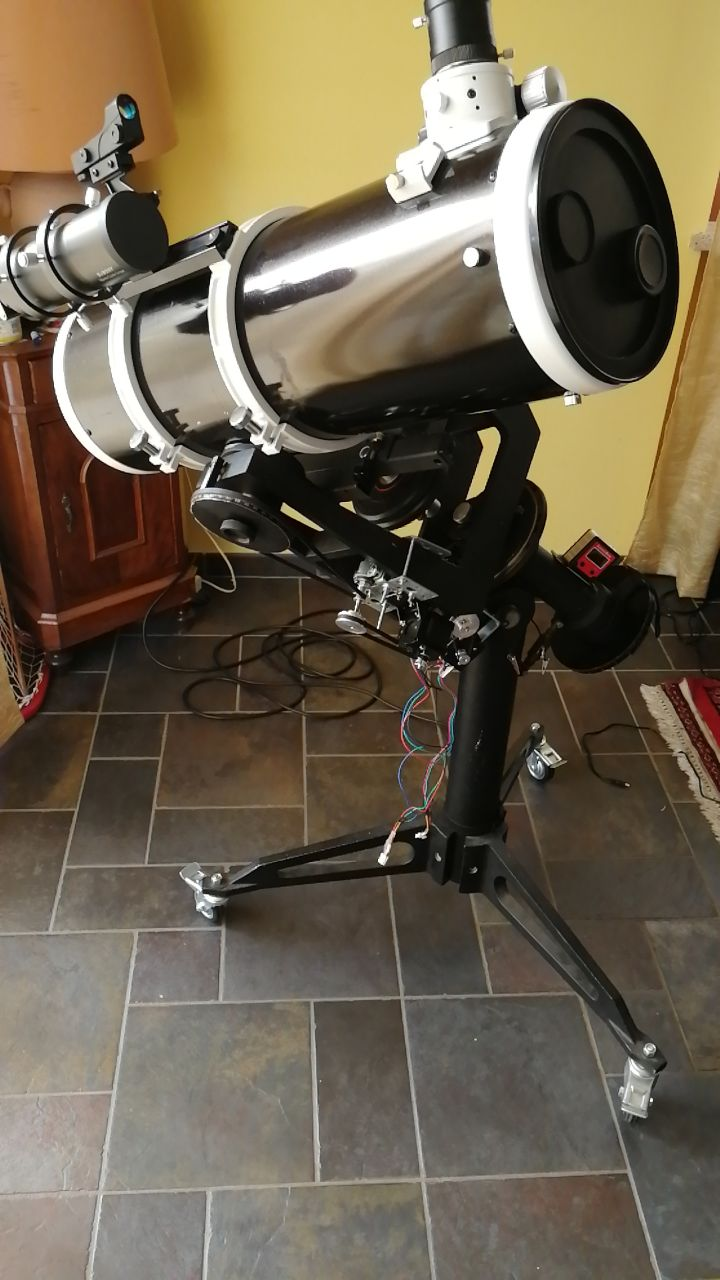
\includegraphics[scale=0.2]{telescope_image.jpg}
    % \end{minipage}

    \begin{multicols}{2}

        \tableofcontents

        \begin{minipage}{0.5\textwidth}
            \centering
            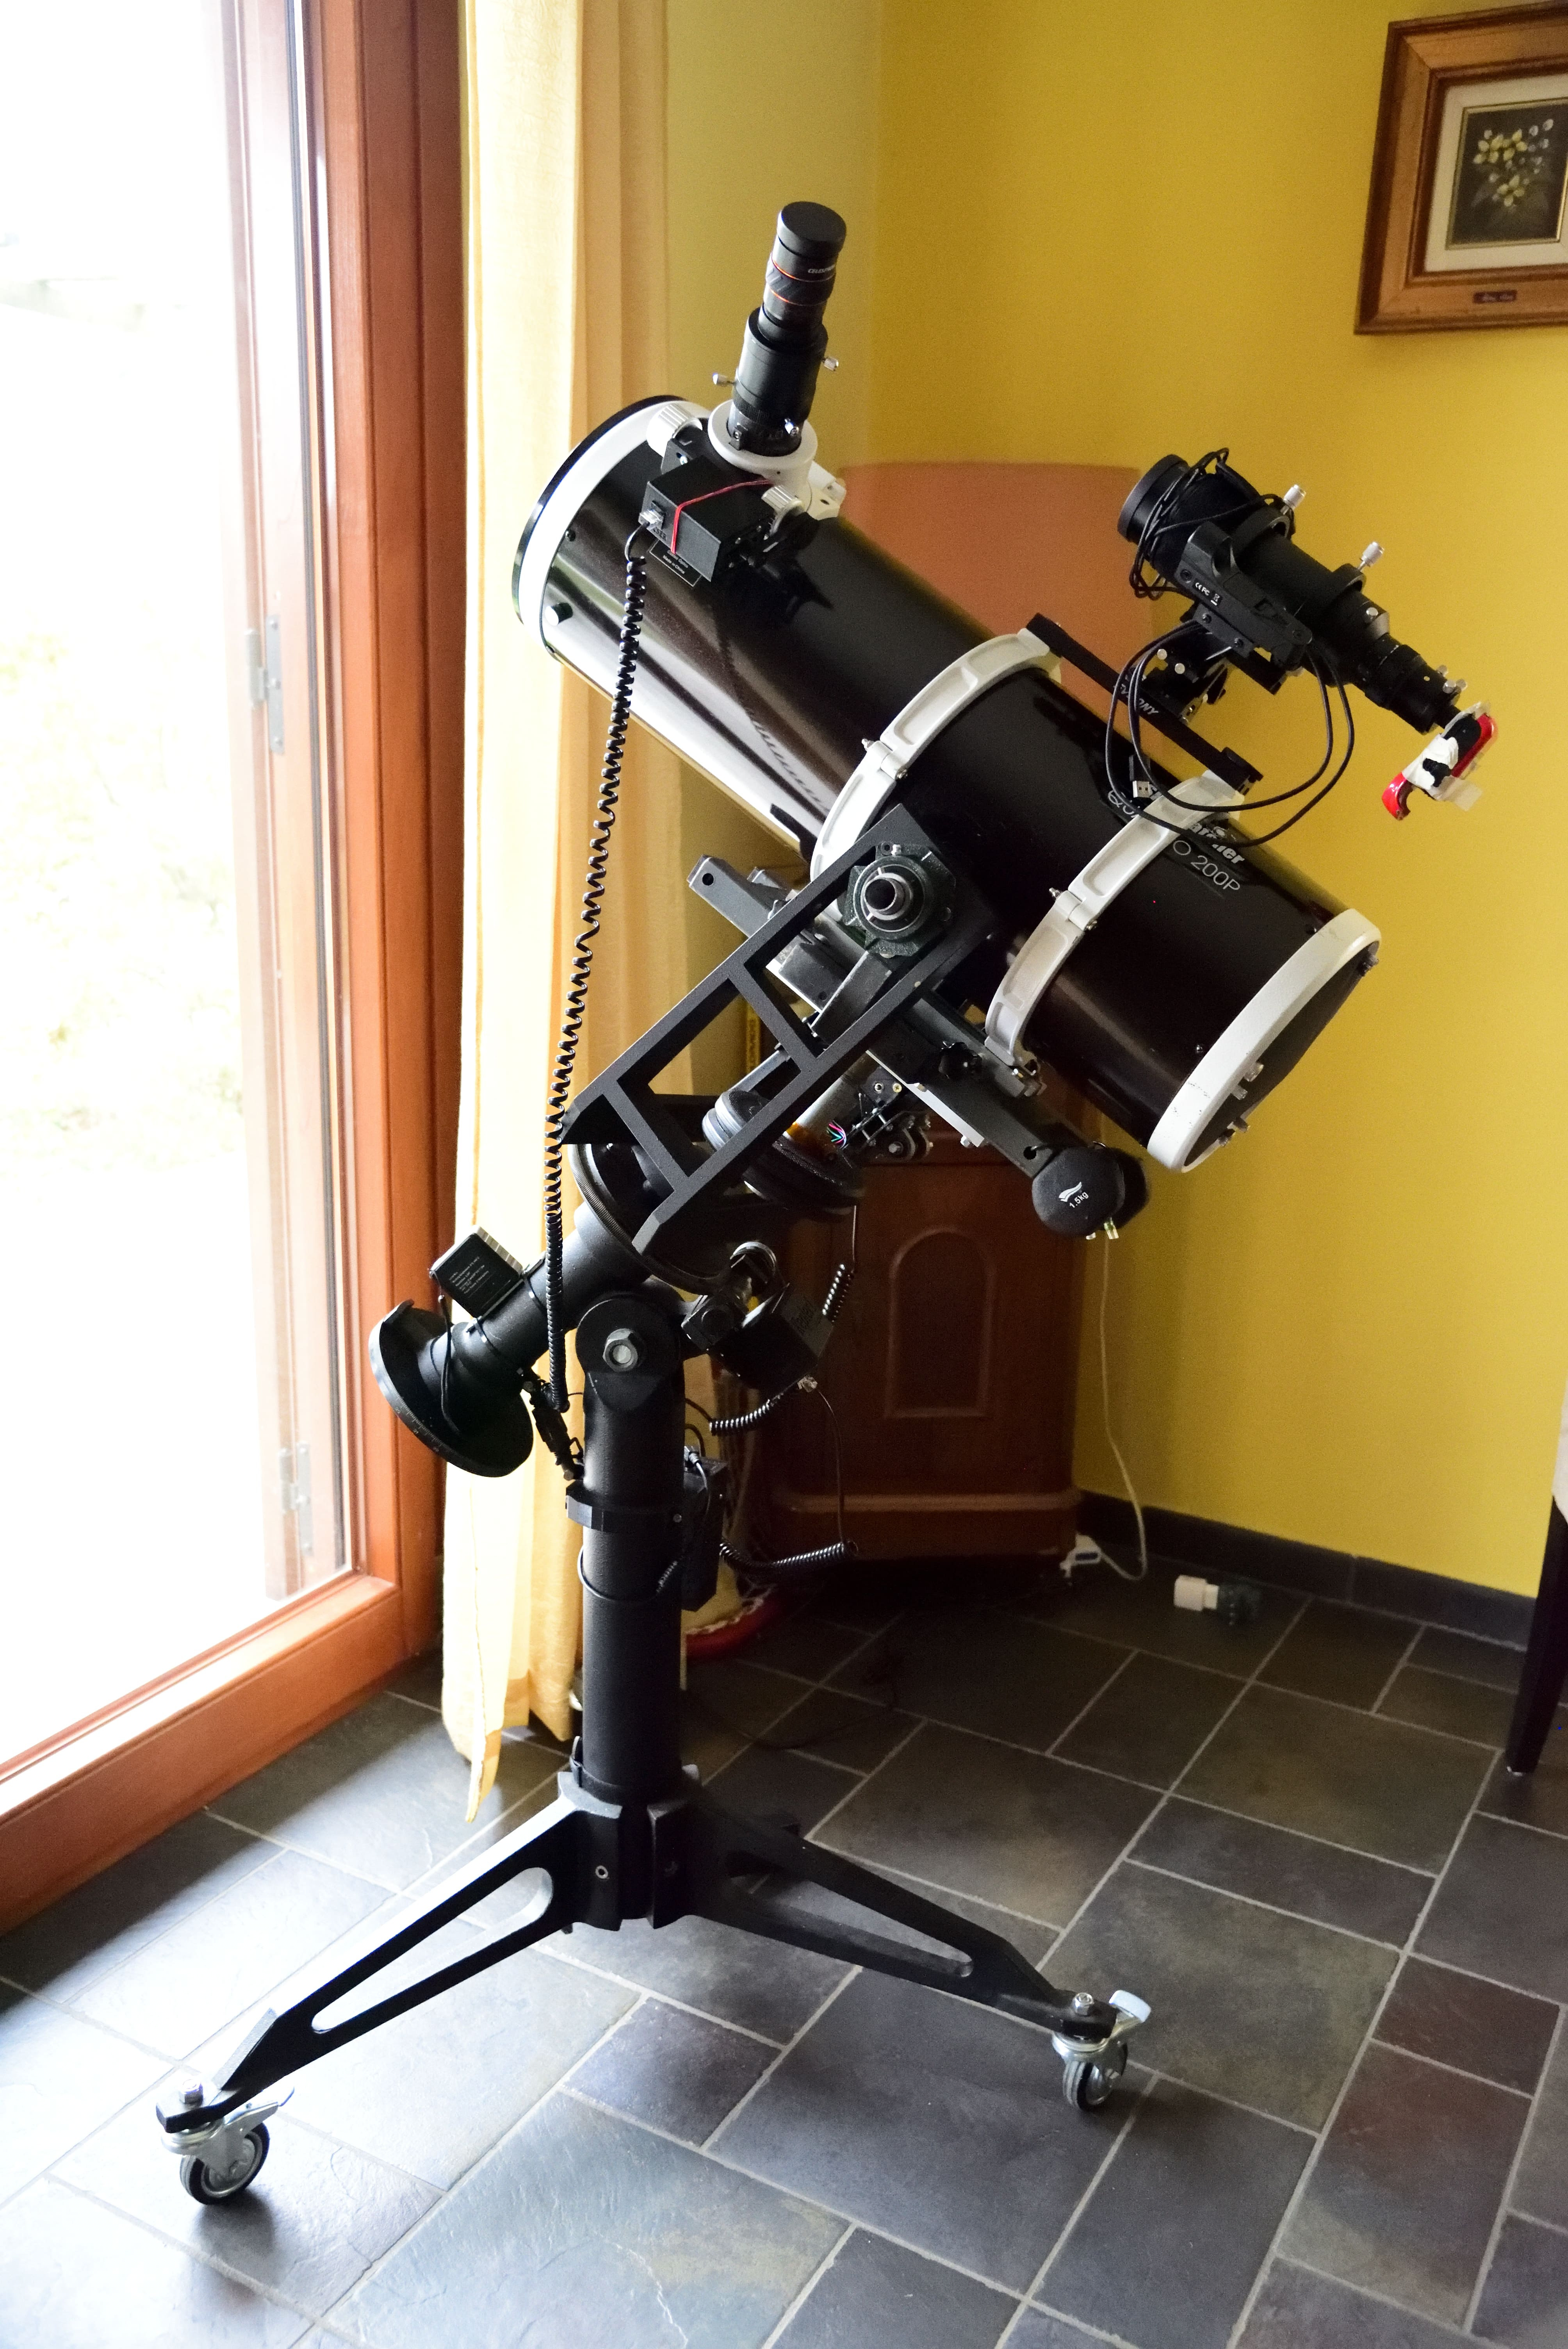
\includegraphics[scale=0.2]{DSC_5264_00001.jpg}
            \captionof{figure}{Final result: our brand-new telescope.}
        \end{minipage}

        \section{Telescope Description}
        The starting point of the project is of course the telescope.
        In our garage, for many years, a 1980 Urania telescope has eaten a lot of dust.
        The telescope's mirror resent of years in humidity and temperature jumps in the garage.
        In the beginning, we have cleaned the silvered-mirror with soap and water, but the silver still seemed to be a bit compromised.
        We do not talk long about this telescope, since we have soon substituted it with a brand-new Skywatcher Quattro.
        The latter is placed on the Urania mount, since it is still a nice mount and, in our advice, has still not surpassed robustness.
        Indeed, the mount is a very heavy (telescope and mount totally weight 20kg!) equatorial and motorized (still works!) mount.
        
        For our money, but most importantly for our fun and entertainment, we decided to modernize our old telescope.

        \subsection{Urania telescope}
        We briefly add the specifics of the old Urania telescope, as a sort of respect for many years of honorable work before the deep dark in the garage.
        \\
        \begin{minipage}{0.5\textwidth}
            \centering
            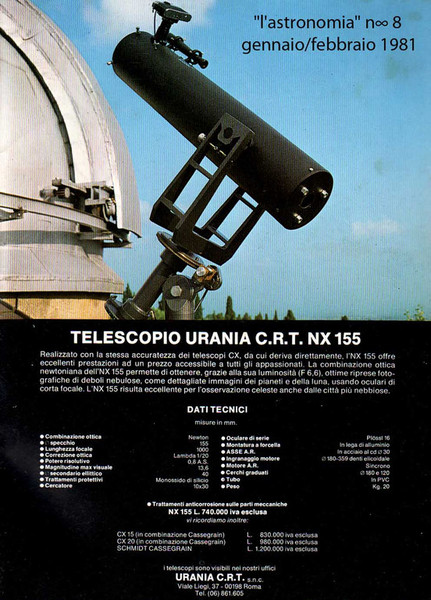
\includegraphics[scale=0.4]{urania_upper.jpg}
            \captionof{figure}{Urania telescope and mount.}
            \label{fig:urania_telescope_mount}
        \end{minipage}
        \\
        The telescope is a Urania C.R.T. NX 155, as the one in figure \ref{fig:urania_telescope_mount}.
        \\
        \begin{minipage}{0.5\textwidth}
            \centering
            \begin{tabular}{c|c}
                Specific name & value \\
                \hline
                type & reflector \\
                technique & Newton  \\
                material & PVC  \\
                weight (kg) & 10 \\
                aperture (mm) & 155 \\
                focal length (mm) & 1000 \\
                focal & f/6.5 \\
                resolution power & 0.8 \\
                limit magnitude value (mag) & 13.6 \\
                Mirror Treatment & Silica monoxide \\
                \hline
            \end{tabular}
            \captionof{table}{Urania C.R.T. NX 155 specifics.}
        \end{minipage}

        \subsection{Telescope's mount}
        The telescope is place onto an aeronautic Aluminum tripod equatorial mount.
        \\
        \begin{minipage}{.4\textwidth}
            \begin{tabular}{cc}
                Specific & value \\
                \hline
                weight (kg) & \\
                type & fork \\
                material & Aluminum alloy \\
                RA axis diameter (mm) & 30 \\
                RA axis material & cadmium steel \\
                RA motor & 3W synchronous \\
                \hline
            \end{tabular}
            \captionof{table}{Urania's mount specifics.}
            \label{tab:mount}
        \end{minipage}

        Starting from the bottom: three pods of 30cm depart from a central post. Each one has a wheel which permits the structure to move freely and then to fix the position using stops.
        The central post terminates with the second axis holder at an inclination equal to the Earth's ecliptic \(23.43^{\circ} = 23^{\circ} 26'\).

        This axis must be aligned with the Polar star (labelling the North).
        In this way, a 3W synchronous motor can follow the sky movement.

        Departing from this second axis, a two-arms fork is free to rotate around two degrees-of-freedom defining the right ascension (RA) and the declination (DEC).
        The two arms are separated by the distance \(d = 15\)mm which is the Urania telescope aperture.
        \subsection{Skywatcher 8P Quattro telescope}
        Skywatcher 8P Quattro Newtonian telescope (figure \ref{fig:skywatcher_telescope_mount}) offers an optimal astrophotography performance.
        For this reason we have decided to substitute the Urania telescope with this brand-new Skywatcher telescope.
        \\
        \begin{minipage}{0.5\textwidth}
            \centering
            \begin{tabular}{c|c}
                Specific name & value \\
                \hline
                type & reflector \\
                technique & Newton  \\
                material & Carbon  \\
                weight (kg) & 8.0 \\
                aperture (mm) & 200 \\
                focal length (mm) & 800 \\
                focal & f/4 \\
                resolution power & 0.58 \\
                limit magnitude (mag) & 13.3 \\
                collect light & 820 \\
                magnification & 400 \\
                Mirror Treatment & Aluminum Coating \\
                Focuser & Crayford dual-speed 50.8/31.8 \\
                \hline
            \end{tabular}
            \captionof{table}{Skywatcher 8P Quattro}
            \label{tab_skywatcher_quattro}
        \end{minipage}
        \\
        \begin{minipage}{0.5\textwidth}
            \centering
            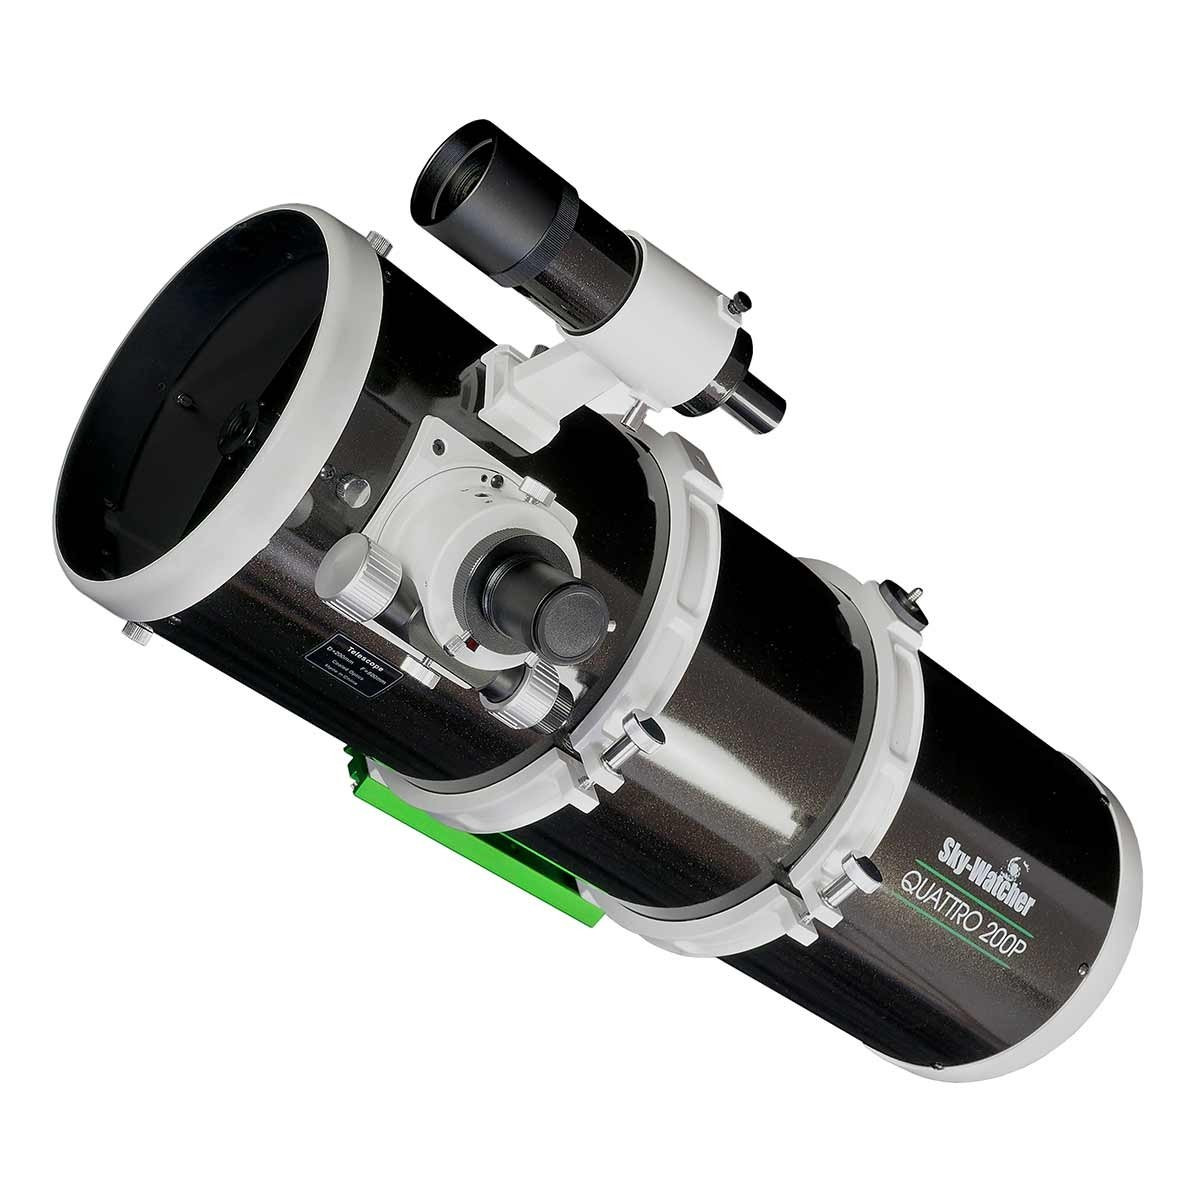
\includegraphics[scale=0.2]{newton-quattro-200-sky-watcher.jpg}
            \captionof{figure}{Skywatcher Quattro telescope.}
            \label{fig:skywatcher_telescope_mount}
        \end{minipage}
        \\
        Since the Skywatcher telescope does not fit in the fork, we have thought to build a "saddle" onto which placing the telescope.
        The specifics of this installation are shown in the following section.
         

        \section{Telescope substitution: from Urania's tube to Skywatcher's tube}
        Passing from the Urania telescope to Skywatcher telescope we have faced the problem of how to insert the latter in the telescope mount.
        Indeed, since Skywatcher's telescope diameter is 200mm it does not fit inside the mount fork.

        Our solution is to insert a seat in which to place the telescope.
        The barycenter of the telescope is not centered with the DEC axis, thus we have settled a post capable of holding weights to balance the forces.
        See figure \ref{fig:piastra_DEC} and \ref{fig:piastra_particular}.
        \\
        \begin{minipage}{0.25\textwidth}
            \centering
            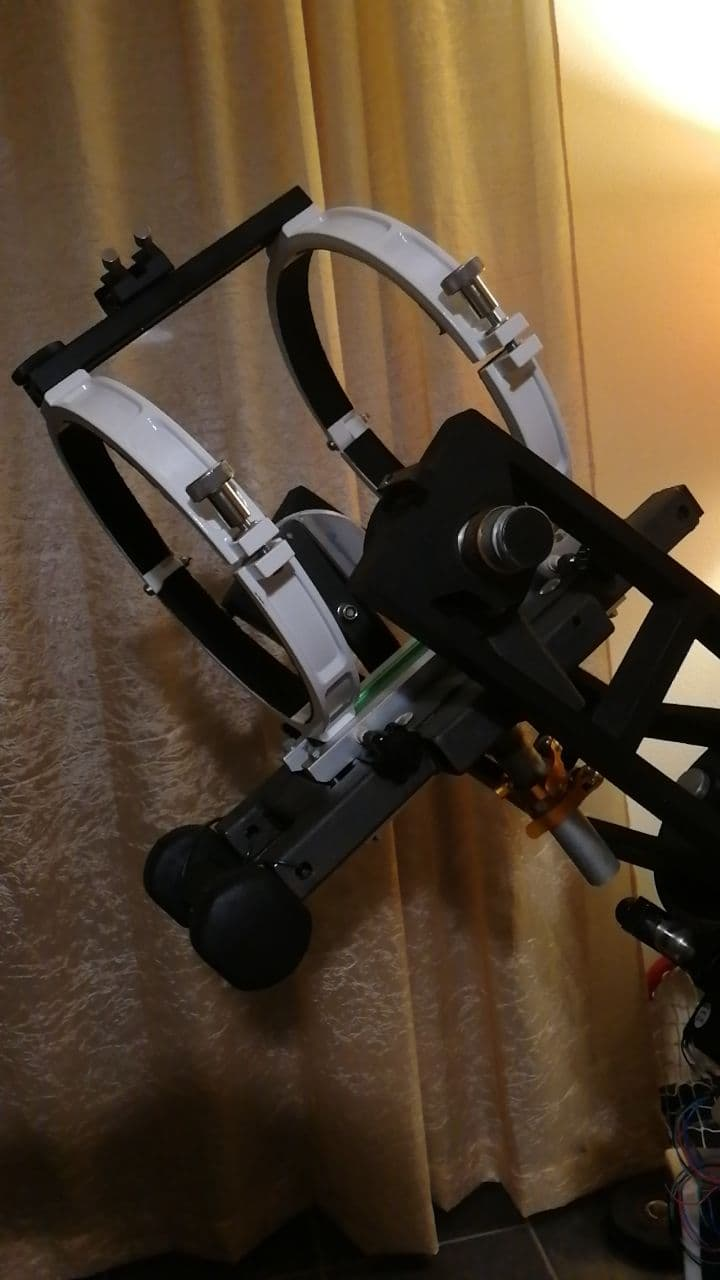
\includegraphics[scale=0.5]{DEC_sede.jpg}
            \captionof{figure}{The mechanism built to insert Skywatcher's telescope into the Urania robust mount.}
            \label{fig:piastra_DEC}
        \end{minipage}
        \begin{minipage}
            {0.25\textwidth}
            \centering
            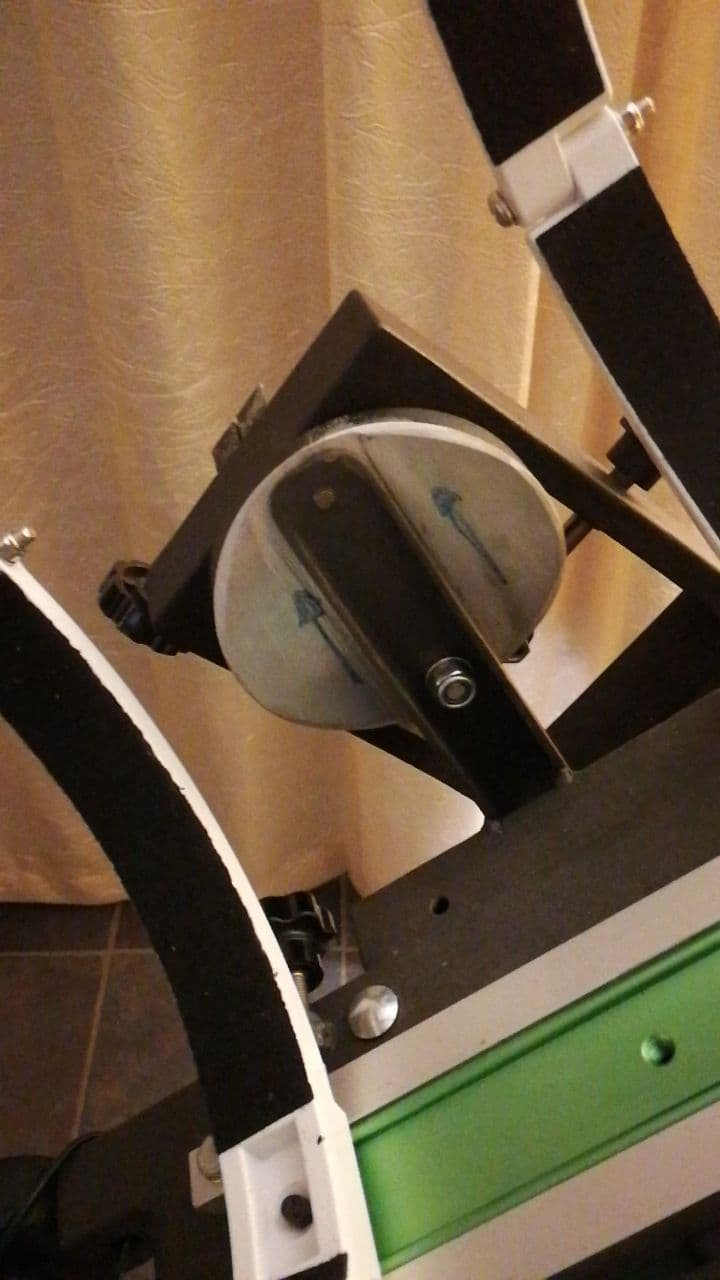
\includegraphics[scale=0.5]{DEC_piastra.jpg}
            \captionof{figure}{detail of the replacement plate that supports the new telescope.}
            \label{fig:piastra_particular}
        \end{minipage}
        \\
        The scheme with distances is visible in figure \ref{fig:DEC_piastra_dimensioni}.
        \\
        \begin{minipage}
            {0.5\textwidth}
            \centering
            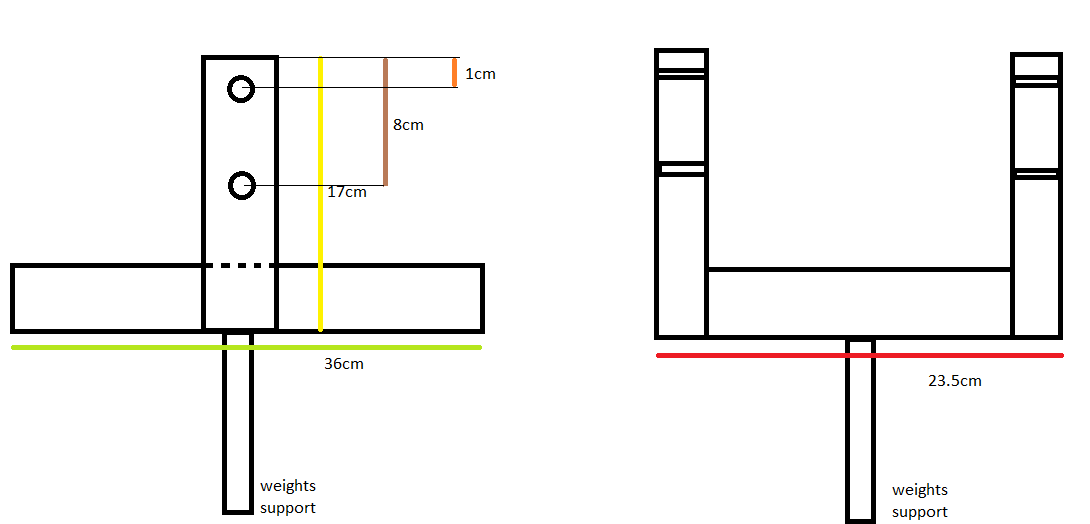
\includegraphics[scale=0.75]{DEC_piastra_dimensioni.png}
            \captionof{figure}{Schematic view of the telescope mount insertion.
            This represents only the installation build with some squared metal bars upon which the two white loops (which hold the telescope tube) are fixed and are not illustrated in this scheme. The two holes in each arm serve to fix the structure on the mount. }
            \label{fig:DEC_piastra_dimensioni}
        \end{minipage}

        Lastly, to enhance the fluidity of motion and reduce the backlash, the rotation mechanism is enriched with a system of two bearing for each fork arm, one interior and one fixed in the mount externally, see figure \ref{fig:cuscinetto-DEC}.
        \\
        \begin{minipage}
            {.5\textwidth}
            \centering
            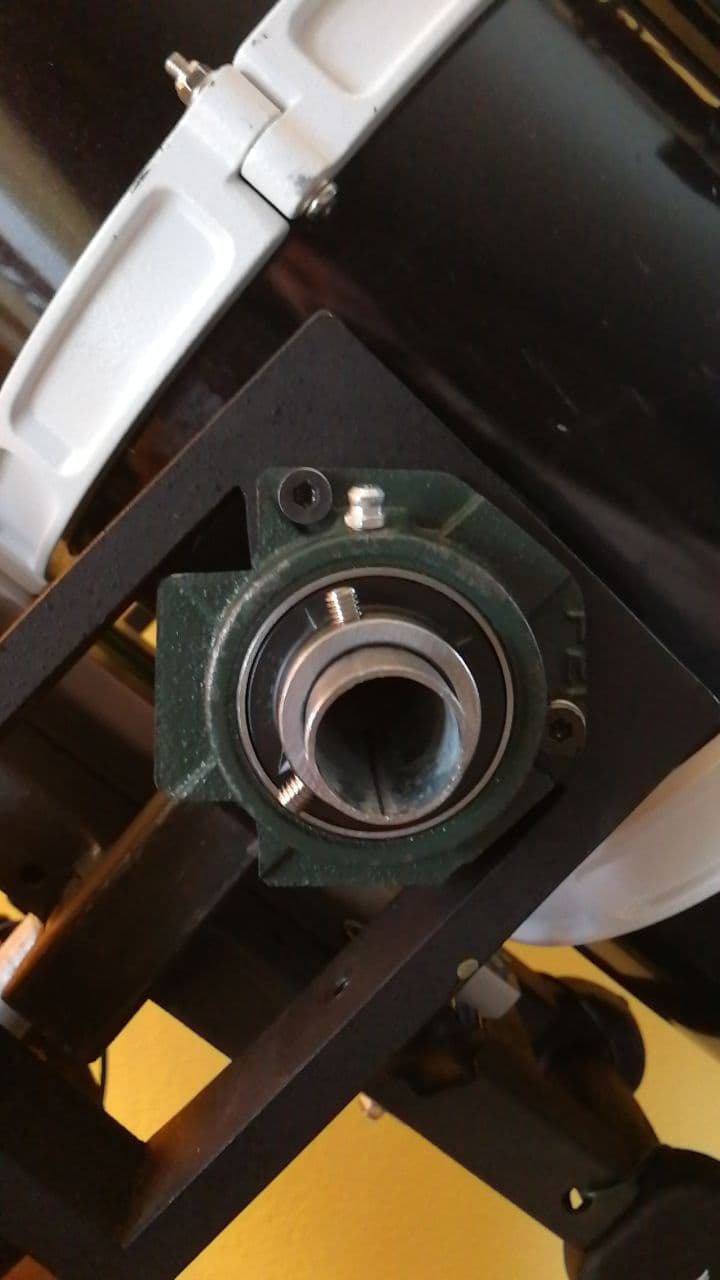
\includegraphics[scale=.45]{cuscinetto-dec.jpg}
            \captionof{figure}{External bearing mounted on one fork arm.}
            \label{fig:cuscinetto-DEC}
        \end{minipage}


         

        \section{Motorization: microcontrollers}
        \subsection{The Arduino experience}
        We decide to write this section more as an advertisement to not follow this way than for other purposes.

        The first, natural, approach was to try to use some at-home-technology.
        Alone on a shelf, an Arduino UNO R3 card was waiting to take part of another project with some friends: a 28BYJ-48 stepper motor and colorful cables.
        What a better occasion to be mounted on the telescope in turns of the 3W motor?

        With some fortunate events, the stepper motor is adapted to the telescope's RA rotating worm shaft.
        Was it good as a tracker motor with a constant motion?
        The answer is no.
        Indeed, some tests revealed bad performances like the inconstant rotation and several stops due to lack of robustness of the motor.
        This result was easily supposed from the beginning, but this try was costs-less, \(i.e.\) free since all the components were at home.
        Indeed, citing Wayne Gretzky:
        \begin{quote}
            "you miss one hundred percent of the shots you don't take",
        \end{quote}
        so it was a matter of must-a-do proof.
        It also gave us the opportunity to face some \textit{engineering} problems.
        
        During a little internet journey, we have found a new stepper motor with a nema 17 standard;
        we have bought two kinds: one of the more robust stepper motors on store and one less robust.
        
        The 28BYJ-48 stepper motor, sadly, returns onto its shelf as, shortly after, would do the Arduino UNO card.

        \subsection{Stepper motors}
        In this subsection we write the specifics of the stepper motors used for the RA and DEC mechanization (for both we have used nema 17 motors) and the focuser (developed with a nema 11 stepper motor).

        % \subsubsection{RA stepper motor}
        \begin{minipage}{0.5\textwidth}
            \centering
            \begin{tabular}{cc}
                \textbf{17HM15-0904S stepper motor}&\\
                Electronics&\\
                \hline
                Manufacturer code & 17HM15-0904S\\
                Engine type & bipolar\\
                Pitch angle (deg) & 0.9 \\
                Torque (Ncm)& 36\\
                Rated current/phase (A) & 0.9\\
                Phase resistance (Ohm)& 60\\
                Voltage (V)& 5.4\\
                Inductance (mH)& 12 \(\pm\) 20\% (1 kHz)\\
                 & \\
                Physical specifications&\\
                \hline
                Frame dimensions (mm\(^2\))& 42x42 \\
                Body length (mm)& 40 \\
                Shaft diameter (mm)& 5 \\
                Stem length (mm)& 22 \\
                D-cut length (mm)& 15 \\
                Number of cables & 4\\
                Lead number (mm)& 300 \\
                Weight (g) & 280\\
                \hline
            \end{tabular}
            \captionof{table}{Nema 17 (0.9A) stepper motor specifics.}
            \label{tab:nema_17_specifics}
        \end{minipage}

        % \subsubsection{DEC stepper motor}
        
        \begin{minipage}{0.5\textwidth}
            \centering
            \begin{tabular}{cc}
                \textbf{17HM19-2004S1 stepper motor}&\\
                Electronics&\\
                \hline
                Manufacturer code & 17HM19-2004S1\\
                Engine type & bipolar\\
                Pitch angle (deg) & 0.9 \\
                Torque (Ncm)& 46\\
                Rated current (A) & 2\\
                Phase resistance (Ohm)& 1.4\\
                Voltage (V)& 2.8\\
                Inductance (mH)& 4\\
                 & \\
                Physical specifications&\\
                \hline
                Frame dimensions (mm\(^2\))& 42x42 \\
                Body length (mm)& 48 \\
                Shaft diameter (mm)& 5 \\
                Stem length (mm)& 24 \\
                D-cut length (mm)& 24 \\
                Number of cables & 4\\
                Lead number (mm)& 500 \\
                Weight (g) & 370\\
                \hline
            \end{tabular}
            \captionof{table}{Nema 17 (2A) stepper motor specifics.}
            \label{tab:nema_17_specifics_2}
        \end{minipage}

        % \subsubsection{Focuser stepper motor}
        \begin{minipage}{0.5\textwidth}
            \centering
            \begin{tabular}{cc}
                \textbf{11HS12-0674S stepper motor}&\\
                Electronics&\\
                \hline
                Manufacturer code & 11HS12-0674S\\
                Engine type & bipolar\\
                Pitch angle (deg) & 1.8 \\
                Torque (Ncm)& 7\\
                Rated current (A) & 0.67\\
                Phase resistance (Ohm)& 5.6\\
                Voltage (V)& 3.8\\
                Inductance (mH)& 4.2\\
                 & \\
                Physical specifications&\\
                \hline
                Frame dimensions (mm\(^2\))& 28x28 \\
                Body length (mm)& 31.5 \\
                Shaft diameter (mm)& 5 \\
                Stem length (mm)& 20 \\
                Number of cables & 4\\
                Lead number (mm)& 300 \\
                Weight (g) & 110\\
                \hline
            \end{tabular}
            \captionof{table}{Nema 11 stepper motor for the focuser motion specifics.}
            \label{tab:nema_11_specifics}
        \end{minipage}

        \subsection{ESP32}
        After buying the new stepper motor, on the internet we have found good impressions on the ESP32 microcontroller.
        ESP32 is a series of low-cost, low-power system on a chip microcontroller with integrated Wi-Fi and dual-mode Bluetooth.
        We've bought the ESP32 D1 R32, the one in figure \ref{fig:esp32}, for better attaching the motor using the CNC shield V3 (which is briefly explained in the following).
        Also, Arduino returned on the self with its friends.

        We bumped into a OnStep project (at \url{https://onstep.groups.io/g/main/wiki/19670}) which an open source software providing the control of four stepper motors (RA, DEC, focuser and rotator for astrophotography), weather sensor handling, Wi-Fi and Bluetooth connection, polar alignment and other nice features.
        We decided to follow the "Wemos R32 and CNC V3" project.
        
        \begin{minipage}
            {.4\textwidth}
            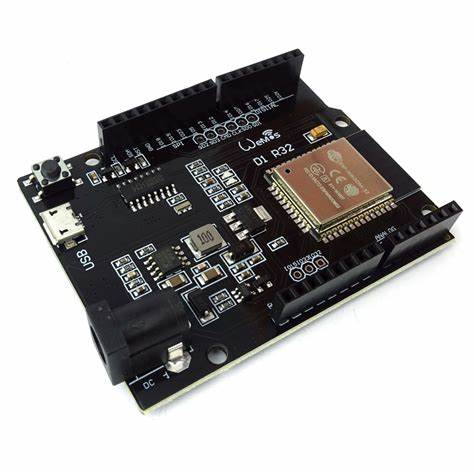
\includegraphics[scale=0.28]{esp32_d1_r32.jpg}
            \captionof{figure}{ESP32 D1 R32 picture.}
            \label{fig:esp32}
        \end{minipage}

        \subsection{CNC Shield V3}
        To better optimize space and wires connections, we have bought a CNC Shield V3 (aka CNC3), see figure \ref{fig:cnc3}.
        \begin{minipage}
            {0.5\textwidth}
            \centering
            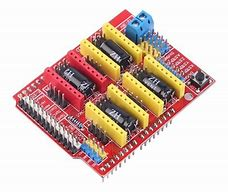
\includegraphics[scale=0.5]{CNC3.jpg}
            \captionof{figure}{CNC3 Shield V3.}
            \label{fig:cnc3}
        \end{minipage}
        It is an add-on shield, built to be used for 3D printers.
        It has 4 slots, each one can host a motor driver.

        \subsection{Motor drivers}
        A stepper motors works only with a driver chip that controls the motor movements.
        Three types of drivers have been used during the configuration of the setup.
        \begin{enumerate}
            \item DRV8828;
            \item TMC2209;
            \item TMC2208.
        \end{enumerate}
        
        In each driver the right amount of current is set, otherwise the stepper motor could work improperly.
        This current depends on the stepper motor current per phase parameter.
        Typically, drivers have a tunable screw for the tension \(V_{ref}\).
        For each type of driver, the formula to calculate the tension \(V_{ref}\) depending on the current/phase are different.\footnote{See \url{https://all3dp.com/2/vref-calculator-tmc2209-tmc2208-a4988/} for more details.}

        The procedure is the following:
        \begin{itemize}
            \item rotate the screw in the counter clock direction;
            \item using a multimeter, check that the tension is zero;
            \item slightly rotate the screw until the tension is the desired one.
        \end{itemize}
        We recommend reducing the theoretical value by a 10\%-30\% to prevent motor dangers.

        \subsubsection{DRV8825}
        For these drivers the tension to be set is roughly the half of the value of the nominal current/phase of the motor.
        For example, if the motor has a current/phase \(1\)A, the tension would be \(0.5\)V.

        \begin{minipage}
            {.4\textwidth}
            \begin{tabular}{cc}
                Current phaser (A) & Current (A) \\
                \hline
                0.90 & 0.45 \\
                2.00 & 0.90             
            \end{tabular}
            \captionof{table}{DRV8828 drivers setup current. Note that we have set a value smaller than the one calculated to prevent motor to break.}
            \label{tab:drivers_curr}
        \end{minipage} 

        \subsubsection{TMC2208 and TMC2209}
        For these drivers the tension value is roughly the same of the current/phase value, \textit{e.g.} if \(I=1\)A the tension would be \(V_{ref}=1\)V.
        Be aware that the TMC2208 has a maximum current output of 1.2A.

        The calculation is 
        \[\frac{I}{\sqrt{2}}=\frac{325mV}{110m\Omega+20m\Omega}\cdot\frac{1}{\sqrt{2}}\cdot\frac{V_{ref}}{2.5V}\Rightarrow V_{ref} = I \cdot 1\Omega.\]
        Remember to reduce to value by a 10\%-30\%.

        \begin{minipage}
            {.4\textwidth}
            \begin{tabular}{ccc}
               Driver & Current/phase (A) & Current (A) \\
                \hline
               TMC2208 & 0.90 & 0.81 \\
               TMC2208 &  2.00 & 1.63 \\                
               TMC2209 (focuser) &  0.67 & 0.50                
            \end{tabular}
            \captionof{table}{DRV8828 drivers setup current. Note that we have set a value smaller than the one calculated to prevent motor to break.}
            \label{tab:drivers_curr}
        \end{minipage} 



        \subsection{Power supply}
        The power supply is provided by a 19V 5A power supply as in table \ref{tab:power_supply}.

        \begin{minipage}
            {.4\textwidth}
            \begin{tabular}{cc}
                 voltage output (V) & current output (A) \\
                 \hline
                19.3 & 4.74 \\
            \end{tabular}
            \captionof{table}{Nominal tension and current outputs of the power supply.}
            \label{tab:power_supply}
        \end{minipage}

        For our initial purposes it was enough, indeed 5A are enough to feed quite well two stepper motors and a poor electronics.
        A rough estimation poses 1.8A for DEC motor, 0.9A for RA motor and few milliampéres for the ESP32. 
        The reader is strongly encouraged to check the total current its circuit needs before buying a power supply.

        \subsection{Sensors: Wi-Fi connection, Real time clock (RTC) and weather sensor (BMP280)}
        An ESP8688 WeMos D1 mini is connected to the CNC3 as shown in \url{https://onstep.groups.io/g/main/wiki/19670}.

        This OnStep has a software addon called the Smart Web Server (SWS) which provides WiFi or Ethernet connections over IP.
        Many devices support this type of connection including cell-phones, tablets, laptop/desktop computers, etc.
        Using this library, it is possible to use programs such as Stellarium via ASCOM drivers provided by the OnStep project \url{http://www.stellarjourney.com/index.php?r=site/software_telescope}.

        \section{Motorization: the mechanics}
        The motorization of the telescope passes through two mechanics adjustments:
        \begin{enumerate}
            \item motorize the RA movement, exploiting the native tracker mechanism;
            \item motorize the DEC movement, which natively has no gears.
        \end{enumerate}

        \subsection{RA motorization}
        The telescope's mount has already a tracking mechanism motorized by a 3W synchronous motor.
        So, in principle, it is only a matter of substitute this old motor, with a new programmable stepper motor.

        The gears are composed by:
        \begin{itemize}
            \item a 359 teeth stage (1 tooth for each degree, fantastic);
            \item an endless screw (worm) mounted on a shaft through a clutch.
        \end{itemize}
        Using this structure, for a continuous sky tracking, the elder motor would complete a round of the worm in 4 minutes.
        Thus, this mechanism rotates the mount with the velocity of a degree in 4 minutes (which is the velocity of the sky moving away in the night).

        We have reduced the ratio by a third adding two other gears (see figure \ref{fig:RA_mechanization}): 60 teeth gear positioned in the shaft and a 20 teeth gear on the motor shaft.
        \\
        \begin{minipage}{.4\textwidth}
            \begin{tabular}{cc|c}
                ratio gear 1 & ratio gear 2 & total ratio \\
                \hline
                1/360 & 1/3 & 1/1080 \\
                \hline
            \end{tabular}
            \captionof{table}{Total reduction of RA mechanization.}
            \label{tab:RA_mechanization}
        \end{minipage}
        \\
        \begin{minipage}{.4\textwidth}
            \centering
            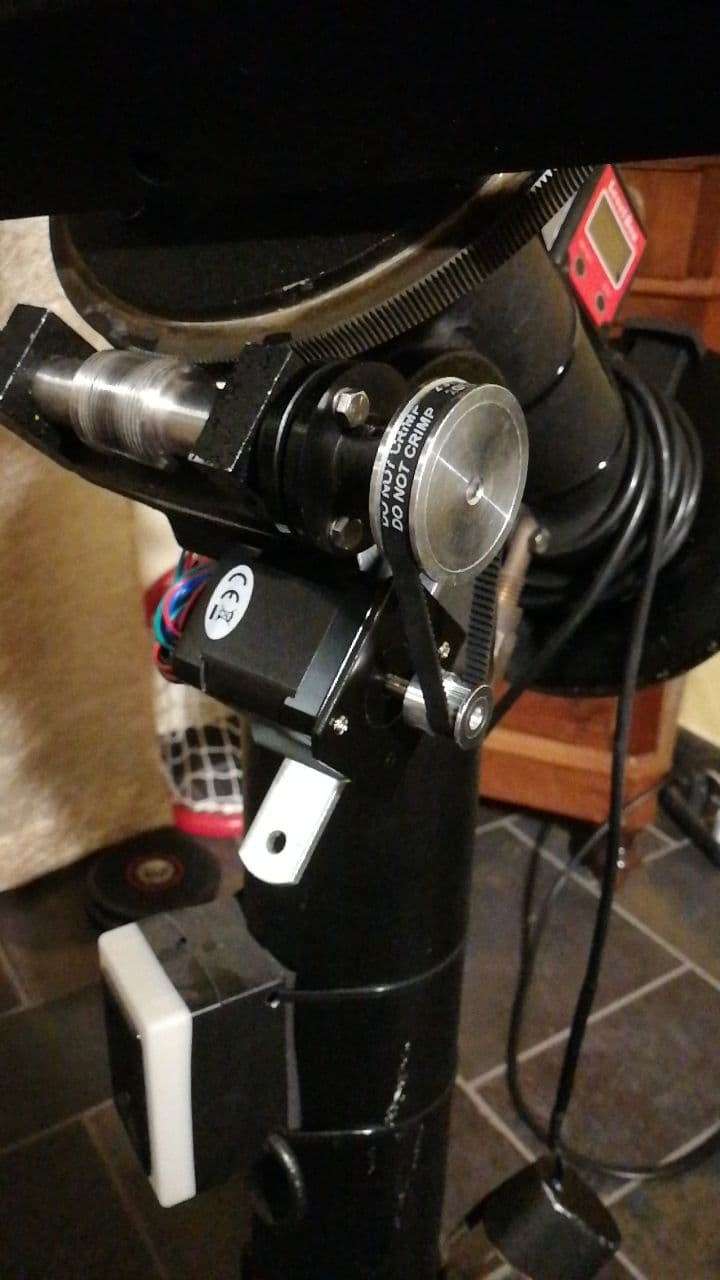
\includegraphics[scale=0.6]{RA_motorization.jpg}  
            \captionof{figure}{Nema 17 stepper motor and gear adjustment.}
            \label{fig:RA_mechanization}         
        \end{minipage}
        \\
        We have choose to install a nema 17 stepper motor with the specifics in table \ref{tab:nema_17_specifics}

        \subsection{DEC motorization}
        The mechanization of the DEC axis was a bit more complicated since there was not a built-in gear to use.
        We tried different versions.
        A first successfully try was to exploit a stand-alone disk.
        On the edge of the latter are present some ticks and grades: it was used a declination angle teller.

        As told above, we have tried different configurations but same stepper motor is used.

        \subsubsection{DEC V1}
        The first version is made using the built-in graded disk mounted on the telescope.
        On this, is attached a 32cm long chain strip.
        Then, a 1/3 reduction shaft is positioned between the first gear and the stepper motor's gear.
        The total reduction with all gear specifics is reported in table \ref{tab:DEC_gear_spec}.
        Figure \ref{fig:DEC_mechanism} is a picture of the mechanism.

        \begin{minipage}
            {0.5\textwidth}
            \centering
            \textbf{DEC-V1 stages}\\
            \begin{tabular}{ccccc}
                \hline
                Gear number & 1 & 2 & 3 & 4 \\
                number of teeth & 188 & 20 & 60 & 20 \\
                \hline
                total ratio & \(\sim \frac{1}{28}\) &&&
            \end{tabular}
            \captionof{table}{DEC mechanism's gear specifics.}
            \label{tab:DEC_gear_spec}
        \end{minipage}
        \\
        \begin{minipage}
            {0.5\textwidth}
            \centering
            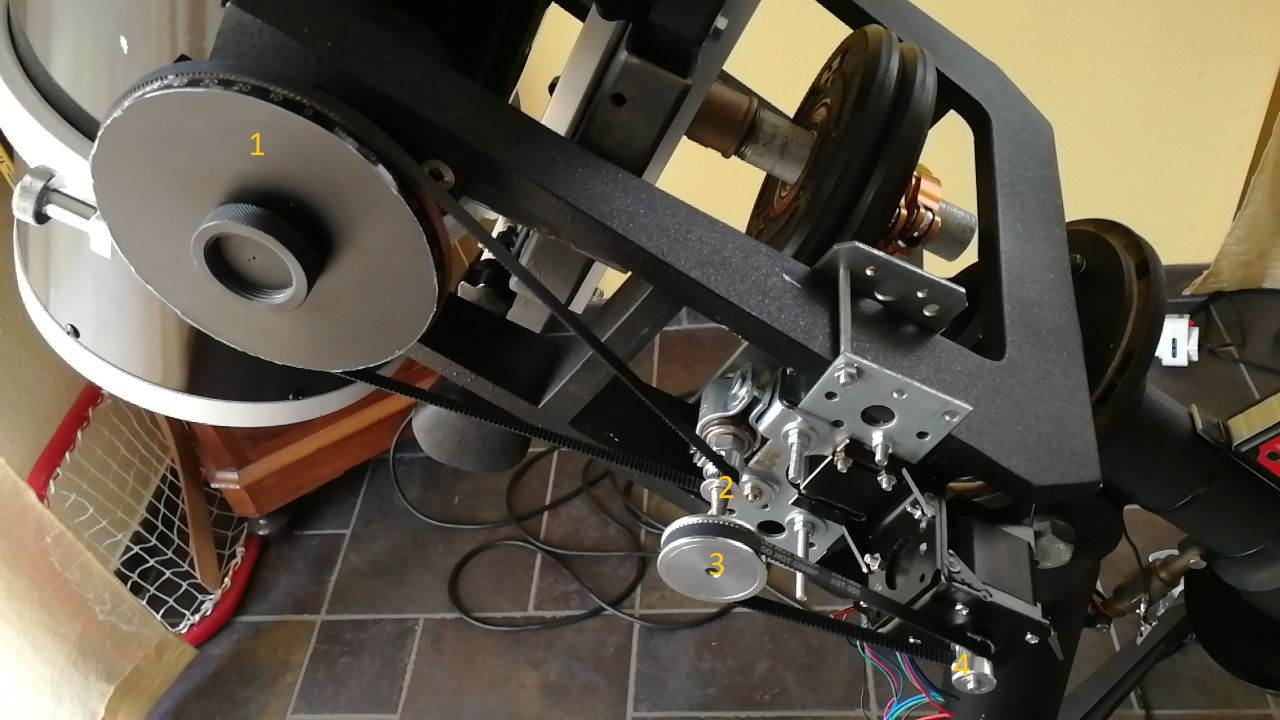
\includegraphics[scale=.28]{DEC_motorization.jpg}
            \captionof{figure}{DEC mechanism.}
            \label{fig:DEC_mechanism}
        \end{minipage}
        \\
        This solution seemed to be efficient, but easy to adjust.
        Also, the stage reduction is too low for a good movement precision.

        \subsubsection{DEC V2}
        The second version made uses again the built-in graded disk mounted on the telescope.
        Also on this construction is glued a 32cm long chain strip.
        Then, a 1/9 reduction is positioned between the first stage and the stepper motor.
        The total reduction with all gear specifics is reported in table \ref{tab:DEC_gear_spec_v2}.
        Figure \ref{fig:DEC_mechanism_v2} is a picture of the mechanism.

        \begin{minipage}
            {0.5\textwidth}
            \centering
            \textbf{DEC-V2 stages}\\
            \begin{tabular}{ccccccc}
                \hline
                Gear number & 1 & 2 & 3 & 4 & 5 & 6\\
                number of teeth & 188 & 20 & 60 & 20 & 60 & 20\\
                \hline
                total ratio & \(\sim \frac{1}{84}\) &&&
            \end{tabular}
            \captionof{table}{DEC mechanism's gear specifics.}
            \label{tab:DEC_gear_spec_v2}
        \end{minipage}
        \\
        \begin{minipage}
            {0.5\textwidth}
            \centering
            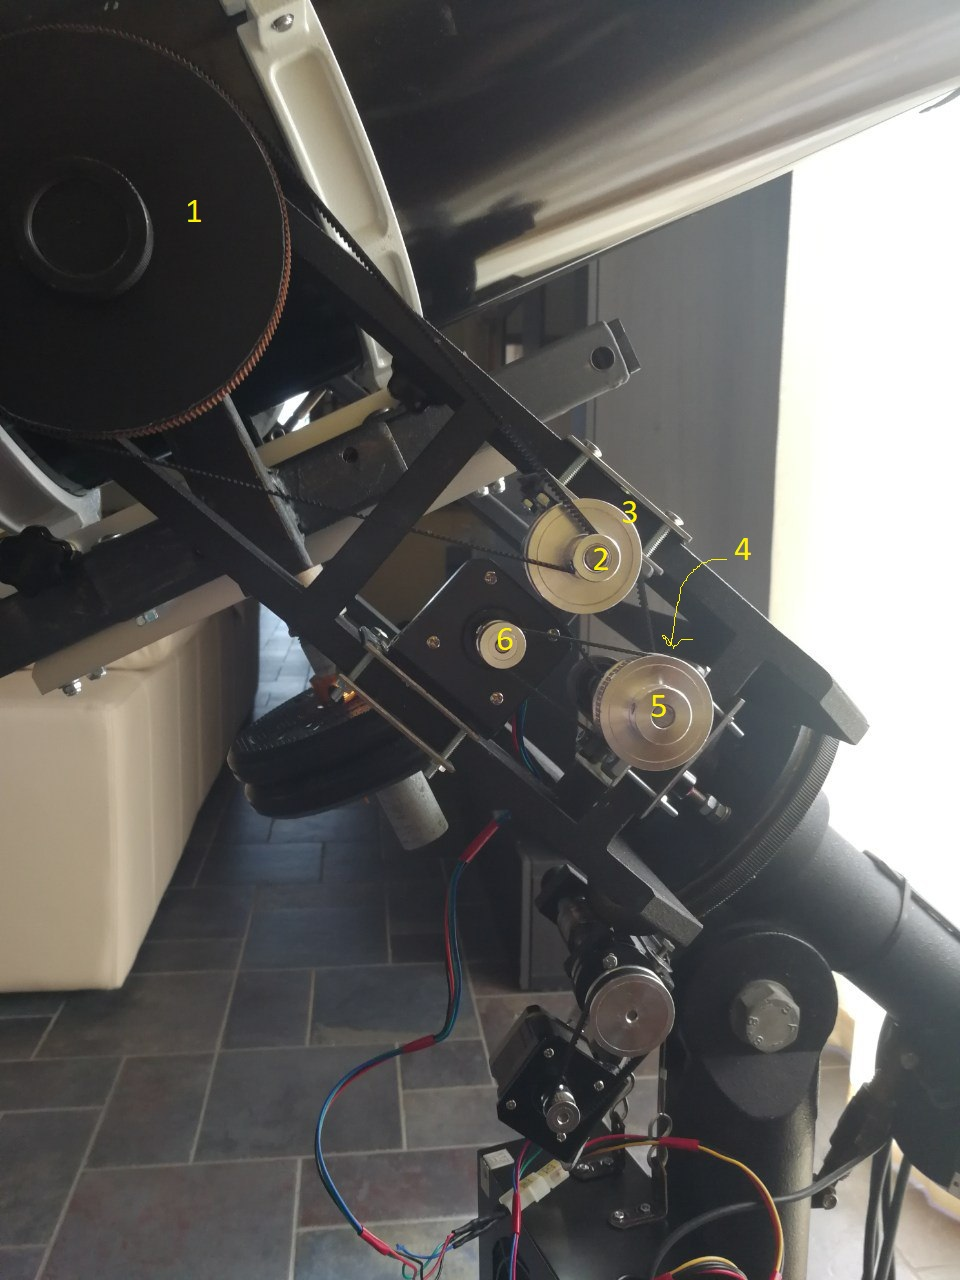
\includegraphics[scale=.2]{DEC_v2.jpg}
            \captionof{figure}{DEC V2 mechanism.}
            \label{fig:DEC_mechanism_v2}
        \end{minipage}
    
        \subsection{DEC V3}
        The third version uses a 3D printed double-belt gear mounted on the telescope.
        Then, a 1/10 ratio is obtained using a worm gear and another 1/3 is obtained between the worm and the final gear.
        The total reduction with all gear specifics is reported in table \ref{tab:DEC_gear_spec_v3}.
        Figure \ref{fig:DEC_mechanism_v3} is a picture of the mechanism.

        \begin{minipage}
            {0.5\textwidth}
            \centering
            \textbf{DEC-V2 stages}\\
            \begin{tabular}{cccccc}
                \hline
                Gear number & 1 & 2 & 3 & 4 & worm\\
                number of teeth & 180 & 30 & 60 & 20 & 10\\
                \hline
                total ratio & \(\sim \frac{1}{180}\) &&&
            \end{tabular}
            \captionof{table}{DEC mechanism's gear specifics.}
            \label{tab:DEC_gear_spec_v2}
        \end{minipage}
        \\
        \begin{minipage}
            {0.5\textwidth}
            \centering
            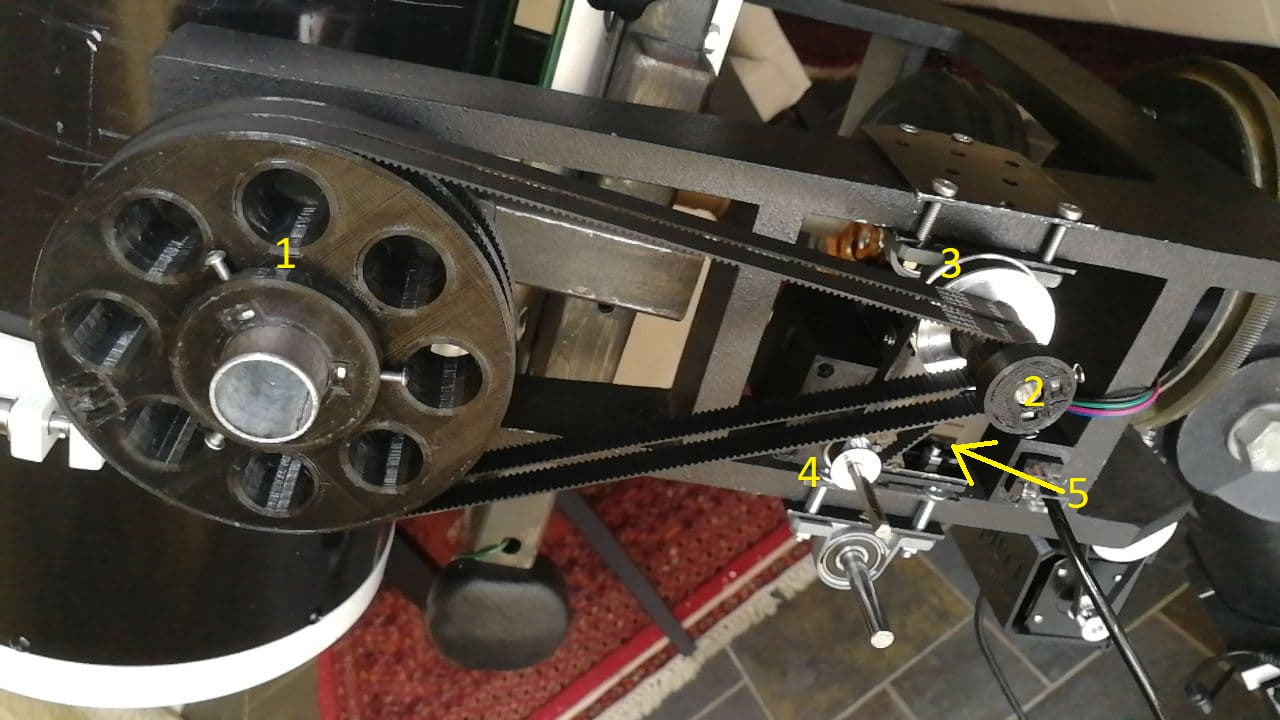
\includegraphics[scale=.6]{DEC-v3.jpg}
            \captionof{figure}{DEC V3 mechanism.}
            \label{fig:DEC_mechanism_v3}
        \end{minipage}

        \subsection{Focuser motorization}
        Another improvement is the motorization of the focuser.
        Using a nema 11 stepper motor, we have created the motor supports and the gears using a 3D printer.
        The reduction stage is 3, see figure \ref{fig:focuser-box}.


        \section{Cable management}
        The wiring between the electronics and the motors is made focusing on the main idea to attach and detach them rapidly.
        We thought to use Ethernet cables.
        They are a versatile solution but how to connect them to the four cables governing the stepper motor?

        Stepper motors have four cables, see figure \ref{fig:stepper-motors-cables}, which have to be driven to the CNC3.
        \\
        \begin{minipage}
            {0.5\textwidth}
            \centering
            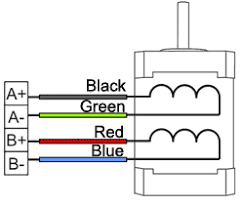
\includegraphics[scale=0.5]{stepper-motors-cables.png}
            \captionof{figure}{Stepper motor cables scheme.}
            \label{fig:stepper-motors-cables}
        \end{minipage}

        \subsection{Ethernet cables}
        Ethernet cables are composed typically by 8 thin cables, each one carrying very few Amperes, approximately \(0.3-0.5A\).
        Since stepper motors require currents of the order of \(1A\), we decided to use them in couple, according to the general Ethernet cabling scheme.
        Thus, the four motor cables are doubled and fixed into the eight way Ethernet socket.

        Then, the main box is prepared to receive the Ethernet cables.
        In the most remote drawers of the garage, we have found an old and burned electronic card with four Ethernet sockets, a power supply entry and an on/off switch.
        Using a multimeter we have checked the pins of each slot and created the connections to the CNC3 shield.

        In figures \ref{fig:box}, \ref{fig:RA-box} and \ref{fig:focuser-box} are shown some examples of Ethernet wiring.

        \subsection{Plastic boxes}
        Using a 3D printer, we have created the focuser motor box with the Ethernet exit, and so we did for the RA motor.
        The microcontroller, the CNC3 shield, the power supply and all the electronics have been thrown in a box.
        The stepper motors drivers after a while become very hot, then we have decided to put a fan in the box.
        In figures \ref{fig:box}, \ref{fig:RA-box} and \ref{fig:focuser-box} are shown the resulting plastic boxes.

        \begin{minipage}
            {0.5\textwidth}
            \centering
            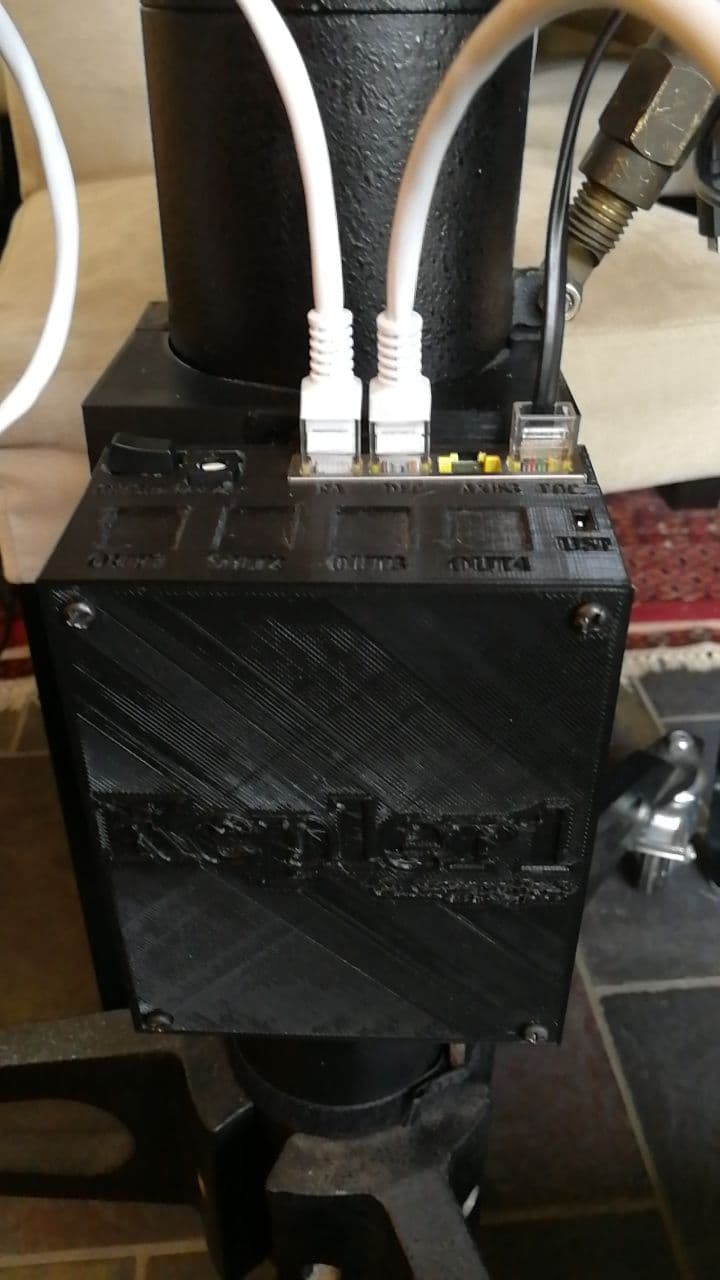
\includegraphics[scale=0.5]{BOX.jpg}
            \captionof{figure}{The main box containing the electronics and its easy management Ethernet connections.}
            \label{fig:box}
        \end{minipage}

        \begin{minipage}
            {0.5\textwidth}
            \centering
            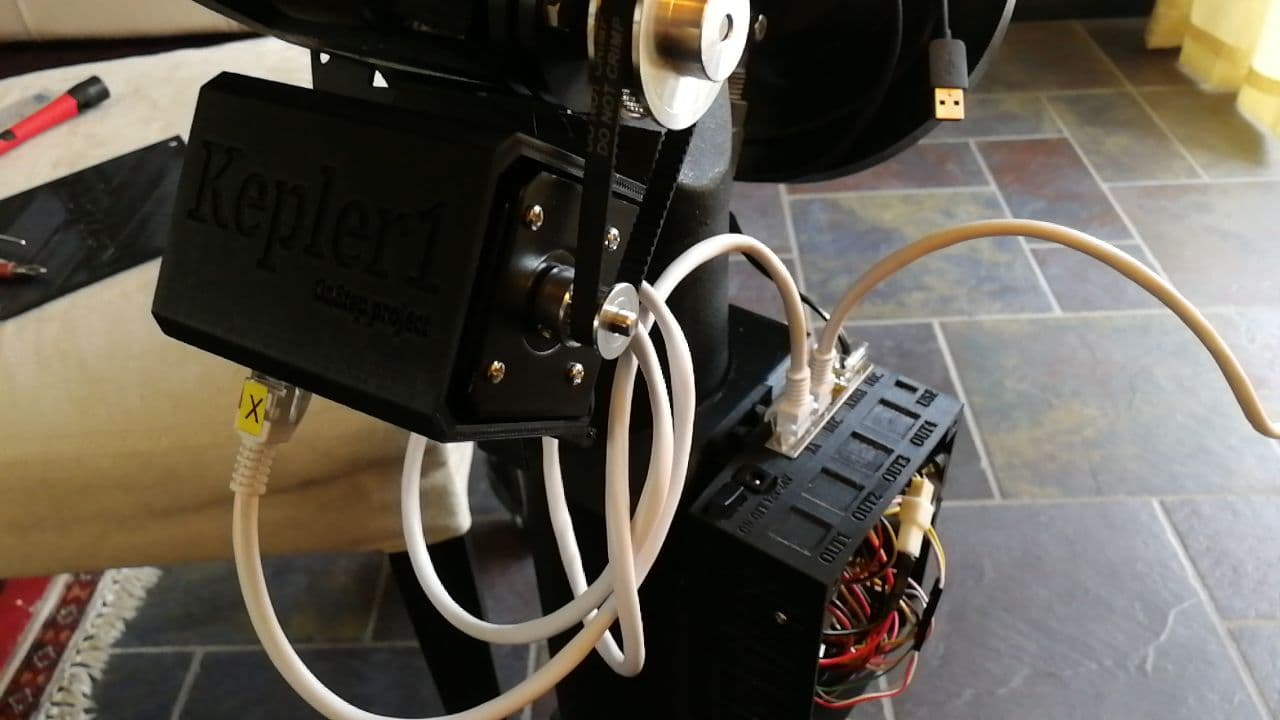
\includegraphics[scale=0.5]{RA-box.jpg}
            \captionof{figure}{The RA motor box containing the stepper motor and its Ethernet socket.}
            \label{fig:RA-box}
        \end{minipage}

        \begin{minipage}
            {0.5\textwidth}
            \centering
            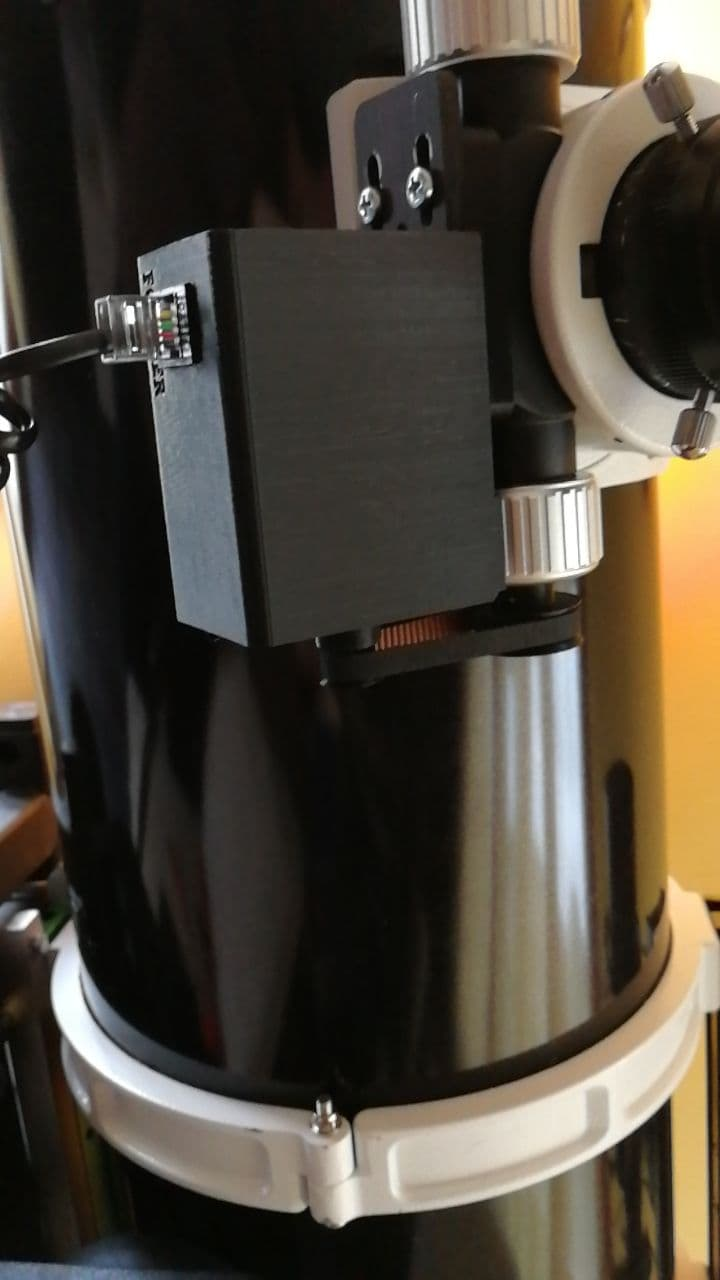
\includegraphics[scale=0.5]{FOCUSER-box.jpg}
            \captionof{figure}{The focuser box containing the focuser stepper motor and its Ethernet socket.}
            \label{fig:focuser-box}
        \end{minipage}

        \section{Tracking}
        Sidereal tracking is done by the OnStep software, of course.
        Otherwise, since the polar alignment may not be perfect we have decided to equip the telescope with an auto-guiding system controlled by the PHD2 app.
        This, in our mind, should optimize the tracking and permits long-exposure photography which is necessary for optimal results.

        Although separated by the previously mechanization, this auto-guiding system interacts with the mount using ASCOM OnStep telescope drivers, and provide corrections to the tracking.
        
        \subsection{Telescope guidescope}
        On the telescope is fixed a 240mm focal length guidescope Svbony SV106.

        \subsection{Guidescope camera}
        The camera is an old red webcam inserted into the guidescope using an adpter.\footnote{See this useful tutorial \url{https://telescopeguides.com/how-to-use-a-webcam-with-a-telescope/}.}

        The result is pretty weird, but it works!
        Just look at the following sections PHD2 logs!

        \section{The software}
        Now comes the software part.
        In our mind, we wouldn't want to spend much time on programming.
        We desired a plug-and-play solution, or something similar.
        A software with easily controlling and possibly which can talk via ASCOM drivers with Stellarium (or others), PHD2 and others astrophotography programs.

        \subsection{OnStep}
        On the internet, we have found a great, open-source, free and customizable software called OnStep.\footnote{Wiki groups:\url{https://onstep.groups.io/g/main/wiki/3860}.\\Github:\url{https://github.com/hjd1964/OnStep}.}
        We have followed the instructions for the WeMos D1 \(+\) CNC V3 project, configured the Config.h file and upload the sketch on the ESP32 board.
        % \begin{minipage}
        %     {0.5\textwidth}
        %     \centering
        %     \begin{tabular}{cc}
        %         Variable & value \\
        %         \hline
        %         \texttt{PINMAP} & CNC3\\
        %         \texttt{SERIAL\_A\_BAUD\_DEFAULT} & 115200 \\
        %         \texttt{SERIAL\_B\_BAUD\_DEFAULT} & 115200 \\
        %         \texttt{SERIAL\_C\_BAUD\_DEFAULT} &  ON \\
        %         \texttt{MOUNT\_TYPE} & FORK \\
        %         \texttt{BUZZER} & ON\\
        %         \texttt{BUZZER\_STATE\_DEFAULT} & ON\\
        %         \texttt{SLEW\_RATE\_BASE\_DESIRED} & 1.0\\
        %         \texttt{TIME\_LOCATION\_SOURCE} & DS3231 \\
        %         \texttt{PPS\_SENSE} & ON \\
        %         \texttt{AXIS1\_STEPS\_PER\_DEGREE} & 38293.333 \\
        %         \texttt{AXIS1\_STEPS\_PER\_WORMROT} & 38400\\ 
        %         \texttt{AXIS1\_DRIVER\_MODEL} & DRV8825\\
        %         \texttt{AXIS1\_DRIVER\_MICROSTEPS} & 32 \\
        %         \texttt{AXIS1\_HOME\_DEFAULT} & 0\\
        %         \texttt{AXIS2\_STEPS\_PER\_DEGREE} & 1002.66667 \\
        %         \texttt{AXIS2\_DRIVER\_MODEL} & DRV8825 \\
        %         \texttt{AXIS2\_DRIVER\_MICROSTEPS} & 32 \\
        %         \texttt{AXIS2\_LIMIT\_MIN} & -35 \\
        %         \texttt{AXIS2\_LIMIT\_MAX} & 80 \\
        %         \texttt{AXIS2\_HOME\_DEFAULT} & 0\\
        %         \texttt{TRACK\_AUTOSTART} & OFF \\
        %         \texttt{BUZZER} & ON \\
        %         \texttt{BUZZER\_STATE\_DEFAULT} & ON\\
        %     \end{tabular}
        %     \captionof{table}{Config.h variables we have changed.}
        %     \label{fig:config_h}
        % \end{minipage}

        Finally, the box is placed on the mount and connected with the Ethernet cables to the motors

        \subsection{PHD2}
        \textit{Push It Dummy-2} is the software that controller the auto-guiding system.
        PHD2 is telescope guiding software that simplifies the process of tracking a guide star, letting you concentrate on other aspects of deep-sky imaging.
        There are plenty tutorials on the internet showing how to use PHD2, so we do not enter so much into details.\footnote{\url{https://www.youtube.com/watch?v=Kd4qzW7uV38} or the pdf \url{https://openphdguiding.org/man-dev/Basic_use.htm}.}
        But we only want to stress out that, after few important configuration passes, the auto-guiding is really simple and promises very good results!

        \subsubsection{Wizard configuration}
        Connection is really simple using the "wizard" option suggested in every tutorials.
        The "unbinned pixel size" is one of the first parameters you have to fix in the wizard which are not quite clear.
        You should be able to get the unbinned pixel size from the camera spec sheet or the manufacturer's web site.
        If this is not the case, you can get the unbinned pixel size by taking the dimension of the sensor and diving it by the number of pixels.

        The "bin level" is the technique to combine proximal bins to form a "superpixel".\footnote{\url{https://www.photometrics.com/learn/imaging-topics/binning-2.}}
        This has the effect of reducing the noise but at the price of reducing the image definition.

        Another remarkable option to fill is the telescope mount's driver, which in this case are the ASCOM OnStep telescope drivers.

        \begin{figure*}[t]
            \centering
            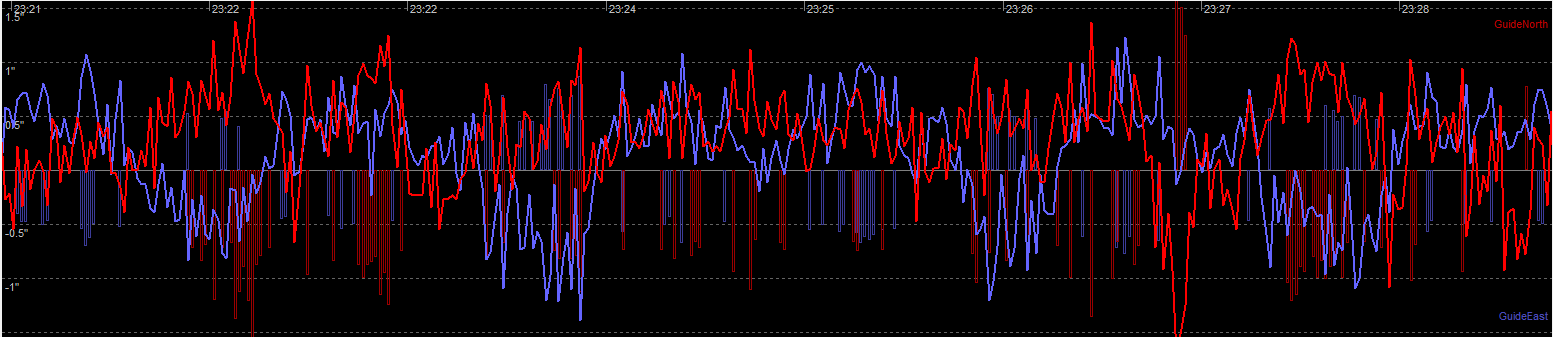
\includegraphics[scale=0.45]{analysis/PHD2/2021-12-09/guide-11-arcsec.png}
            \caption{DEC V3 test: PHD2 log view using arcseconds as units.}
            \label{fig:guide-11-arcsec}
        \end{figure*}
        \begin{figure*}[t]
            \centering
            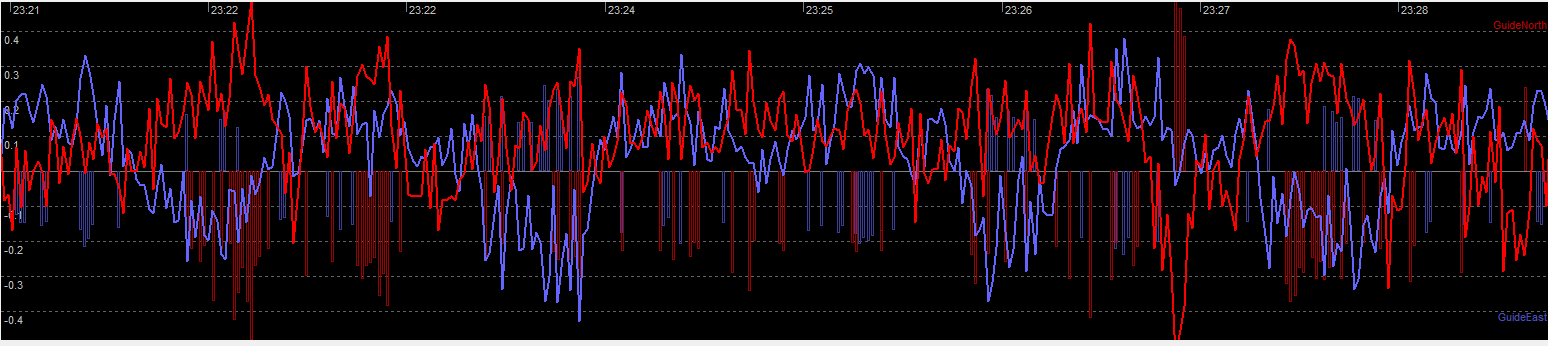
\includegraphics[scale=0.45]{analysis/PHD2/2021-12-09/guide-11-pixel.png}
            \caption{DEC V3 test: PHD2 log view using pixel as units.}
            \label{fig:guide-11-pixel}
        \end{figure*}
        
        \subsubsection{Dark libraries}
        Before starting the first guiding session, it is useful to spend 5 minutes to create a dark library.
        To do so, just press the "Dark" tool on the top and create a new dark library.
        Cover the guidescope, and start the acquisition.

        After the acquisition, remove the cover;
        this should make clearer acquisitions.

        \subsubsection{Connect all!}
        After the configuration, press the first icon in the bottom left and press "connect all".
        Now the camera and the mount are connected to PHD2.

        \subsubsection{Calibration}
        Search a bright star whose declination is between 10 to -10 degrees.
        Start the acquisition pressing the "cycle" icon (the second from the left), then press the "star with a magnifying glass" that selects the most bright star.
        Finally, push the PHD2 icon; this will start the calibration and requires few minutes.

        \subsubsection{Guiding}
        If dark libraries and calibration are done, the guiding can start.
        If it is not present, search in the settings the plot visualization that let you know the adjustments that PHD2 is doing.
        In our case, it is a useful tool to see if our work were precisely enough.        
       
        A useful tool is the "use multiple stars" in the guiding settings.
        The latter permits holding multiple star, and we think this is another improvement to stability in auto-guiding.


        \subsection{Stellarium}
        Stellarium is the software we use to search objects.
        The impressive feature is that, after paring it via ASCOM drivers with the mount, it is possible to tell the telescope to move at the star pointed out in Stellarium.\footnote{See \url{https://www.youtube.com/watch?v=DUdYv311HFw}.}

        The telescope is now free to start few tests to check the goodness of our work!

        \section{Tests}
        \label{sec:tests}
        The test are aimed to estimate the precision of the mount.
        Of particular interest are the test using PHD2 which measure the precision in micro-adjustments for the auto-guiding system.

        The application used to study the PHD2 plots is the PHD2LogViewer app.
        The latter can upload all the guiding session you make, since every session is stored in the PHD2 folder.
        The app also make raw statistical analysis which are good parameters to think about.
        The root-mean-square (RMS) describe the spread of the data points around some average peak value (like standard deviation).
        The value of RMS should be 1 arcsecond or lower for a good guiding.

        \subsection{DEC V3 test}
        The DEC V3 has been developed to reduce the mechanism backlash using the idea "the less the number of belts gets, the better the guiding is".
        The resolution power of the mount is reported in table \ref{tab:resolution-power-DEC-V3}.
        The extrapolated statistics is reported in table \ref{tab:DEC-V3-statistics}.
        \\
        \begin{minipage}
            {.5\textwidth}
            \begin{tabular}{ccc}
                Mechanism & microsteps (x360$^{\circ}$) & resolution (") \\
                \hline
                RA  & 19200 & 0.21\\ 
                DEC & 12800 & 0.65
            \end{tabular}
            \captionof{table}{Resolution power using the DEC V3 mechanism. Microsteps is intended as the total number of microsteps around the entire circumference.}
            \label{tab:resolution-power-DEC-V3}
        \end{minipage}
        \\
        After the calibration, we have pointed the Rosetta nebula and start tracking.
        The result can be seen in figure \ref{fig:guide-11-arcsec} and \ref{fig:guide-11-pixel}.
        \\
        \begin{minipage}{.4\textwidth}
            \centering
            \begin{tabular}{ccc}
                \textbf{Statistics}&RMS&Peak\\
                \hline
                RA& 0.47" (0.15 px)& 1.87" ( 0.58 px)\\
                DEC& 0.90" (0.28 px)&-8.12" (-2.52 px)\\
                Total& 1.02" (0.32 px)&\\
                \\
                \textbf{Drift}& ("/min) & (px/min)\\
                \hline
                RA& +3.01"/min& +0.94 px/min\\
                Dec& +2.14"/min& +0.66 px/min\\
                Polar Alignment Error& 8.7'&\\
                \hline
            \end{tabular}
            \captionof{table}{DEC V3 test: statistics of the guiding.}
            \label{tab:DEC-V3-statistics}
        \end{minipage}


        \section{Conclusion}
        As seen in the test section \ref{sec:tests}, the result are encouraging.
        The auto-guide seem to be stable and quite good since, \textit{e.g.} the RMS is lower than 1 for RA and DEC.
        Photography with this configuration have been set up with more than 2 minutes per pose (which was impossible for us before the devolving of this project).

        As a final consideration, before buying an expensive telescope and mount, consider the idea of converting your own old telescope and the lets play with it! 

    \end{multicols}
\end{document}